\documentclass{llncs}
\usepackage{times}
\usepackage[T1]{fontenc}
\usepackage[utf8]{inputenc}
\usepackage[portuguese]{babel}

\usepackage{epstopdf}
\usepackage{graphicx}
\usepackage{fancyvrb}
\usepackage{amsmath}
\usepackage{listings}
\usepackage{xcolor}

% Configuração do listings
\lstset{
    basicstyle=\ttfamily\small,
    keywordstyle=\color{blue}\bfseries,
    commentstyle=\color{gray}\itshape,
    stringstyle=\color{red},
    breaklines=true,
    frame=single,
    numbers=left,
    numberstyle=\tiny\color{gray},
    captionpos=b
}

\graphicspath{ {./images/} }

% Permitir tableofcontents em LNCS
\setcounter{tocdepth}{3}

\begin{document}
% \mainmatter
\title{Computação Quântica}

\titlerunning{Paper Title}

\author{José Novais}

\authorrunning{José Novais}

\institute{
University of Minho, Department of  Informatics, 4710-057 Braga, Portugal\\
e-mail: a108395@alunos.uminho.pt
}

\date{}
\bibliographystyle{splncs}

\maketitle
\begin{abstract}
     Este trabalho introduz os fundamentos da Computação Quântica, com foco no algoritmo de Grover para busca não estruturada. É apresentada a formulação matemática e a implementação do circuito quântico, analisando a aceleração quadrática obtida. 
\end{abstract}

\renewcommand{\contentsname}{Índice}
\setcounter{tocdepth}{2}
\tableofcontents

\newpage

\section{Introdução}
A computação quântica representa uma mudança de paradigma na ciência da computação, aproveitando os princípios da mecânica quântica para processar informações de maneiras que são fundamentalmente impossíveis para os computadores clássicos. Enquanto a computação tradicional opera com bits em estados binários de $0$ ou $1$, a computação quântica utiliza \textit{qubits}, que podem existir em múltiplos estados simultaneamente. 

Esta característica permite a exploração paralela de soluções. O verdadeiro poder desta tecnologia, no entanto, é revelado através de algoritmos quânticos específicos, desenhados para explorar a interferência quântica e extrair a resposta correta de forma exponencialmente mais rápida ou eficientemente superior aos melhores métodos clássicos conhecidos. Um dos mais proeminentes desta área é o algoritmo de Grover.

\section{O Algoritmo de Grover}
Desenvolvido por Lov Grover em 1996, este algoritmo resolve o problema da busca não estruturada. Em um banco de dados não ordenado com $N$ elementos, um computador clássico precisa, em média, de $N/2$ consultas para encontrar um item específico. O algoritmo de Grover reduz esse tempo para $\mathcal{O}(\sqrt{N})$, oferecendo uma aceleração quadrática através de um processo chamado \textit{amplificação de amplitude}.

A implementação deste algoritmo foi realizada em Python com a biblioteca pennylane que deu suporte ao código das gates e da representação 
visual.

\subsection{A Formulação do Problema de Busca}

Considere uma estrutura de dados não ordenada, análoga a um \textit{array} clássico, onde o objetivo principal é localizar a posição (índice) de um elemento específico que satisfaça uma determinada condição de busca. 

Seja esta estrutura composta por $N$ elementos, onde o tamanho é dado por $N = 2^n$. Essa definição é matematicamente conveniente porque nos permite mapear cada índice do \textit{array}  do intervalo de $0$ a $N-1$ para uma cadeia binária de $n$ \textit{bits}. Em termos de computação quântica, isso significa que podemos representar cada posição da estrutura utilizando os estados da base computacional de um registrador contendo $n$ \textit{qubits}, variando desde o estado $|00\dots0\rangle$ até $|11\dots1\rangle$.

Definimos então $s$ como o índice do \textit{item} específico que estamos buscando (o alvo). Assumimos que a localização de $s$ é completamente arbitrária e desconhecida a priori, sendo um número inteiro que obedece à condição $0 \leq s < N$. 

Para formalizar o processo de busca, introduzimos uma função booleana $f(x)$, que atua como o nosso mecanismo de reconhecimento. Esta função avalia qualquer índice $x$ ($0 \leq x < N$) da seguinte maneira:

\begin{equation}
    f(x) = 
    \begin{cases} 
        1, & \text{se } x = s \text{ (o elemento procurado foi encontrado)} \\ 
        0, & \text{se } x \neq s \text{ (para todos os outros elementos incorretos)} 
    \end{cases}
\end{equation}

\subsection{Implementação do Circuito Quântico}

Para resolver o problema de busca formulado na subseção anterior, traduzimos a função booleana $f(x)$ e a mecânica do algoritmo de Grover para um circuito quântico. 

\subsubsection{Algoritmo de Grover:}

O algoritmo inicia colocando o registrador de entrada (composto por $n$ \textit{qubits}) em uma superposição uniforme de todos os $N$ estados possíveis através da aplicação de portas de Hadamard ($H$). Isso permite que o sistema avalie todas as possibilidades de índices simultaneamente. Em paralelo, um \textit{qubit} auxiliar (\textit{ancilla}) é inicializado no estado negativo $|-\rangle$ por meio de uma porta Pauli-X seguida de uma Hadamard. Este \textit{qubit} extra é a chave para a marcação de fase subsequente.
\begin{figure}[htbp]
    \centering
    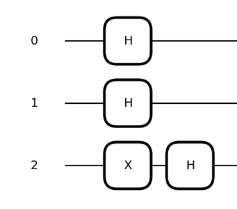
\includegraphics[width=0.4\textwidth]{image.png}
    \caption{Exemplo simples da inicialização com 2 qubits mais 1 de ancilla.}
    \label{fig:minha_imagem}
\end{figure}

\newpage

O \textbf{oráculo} é o segundo passo que atua como a versão quântica da nossa função clássica $f(x)$. No código, sua implementação é realizada através de uma porta Multi-Controlada X. Os \textit{qubits} de entrada atuam como controle e o \textit{ancilla} como alvo. Quando o estado em superposição avaliado corresponde ao índice $s$ procurado (\texttt{ids}), a porta atua. Devido ao fenômeno de \textit{phase kickback} proporcionado pelo estado do \textit{ancilla}, uma fase de $-1$ é transferida exclusivamente para o estado correto $|s\rangle$. Matematicamente, o estado muda de $|s\rangle$ para $-|s\rangle$, efetivamente "marcando" a solução.
\begin{figure}[htbp]
    \centering
    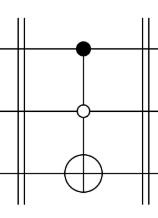
\includegraphics[width=0.2\textwidth]{image2.png}
    \caption{Exemplo da gate de conrolo que só é marcada na solução com o bit de ancilla.}
    \label{fig:minha_imagem}
\end{figure}


A seguir aplicamos o \textbf{operador de difusão}, que realiza uma operação geométrica da reflexão em torno da média. Na implementação, construímos esse operador circundando uma porta Pauli-Z multi-controlada com camadas de portas Pauli-X e Hadamard. O resultado prático desta etapa é a diminuição das amplitudes de probabilidade dos estados incorretos e a amplificação drástica da amplitude do estado marcado $|s\rangle$.

\begin{figure}[htbp]
    \centering
    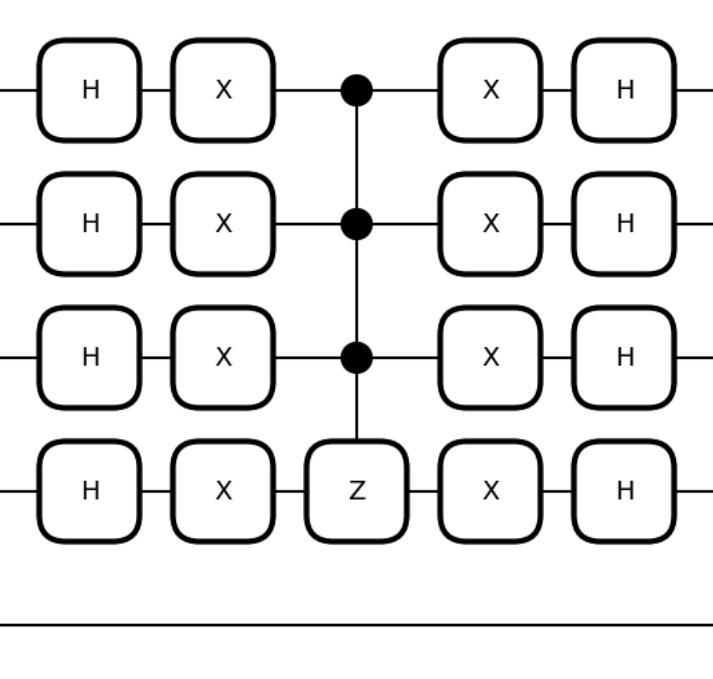
\includegraphics[width=0.5\textwidth]{image3.png}
    \caption{Exemplo da gate de controlo $Z$ que é so feita se todos os qubits estiverem a 0}
    \label{fig:minha_imagem}
\end{figure}

A aplicação combinada de um \textbf{Oráculo e um Operador de Difusão} constitui uma única iteração de Grover. Para maximizar a probabilidade de medir o estado $|s\rangle$ com sucesso, essa rotina deve ser repetida um número específico de vezes. O número ideal de iterações ($R$) depende do tamanho do espaço de busca $N = 2^n$ e é calculado dinamicamente no código através da aproximação:

\begin{equation}
    R \approx \left\lfloor \frac{\pi}{4} \sqrt{2^n} - \frac{1}{2} \right\rceil
\end{equation}

Este algoritmo ja ganha nas iterações de um algoritmo de busca classica com o paralelismo quantico reduzindo a complexidade temporal de $\mathcal{O}(N)$ (necessária em uma busca linear tradicional) para apenas $\mathcal{O}(\sqrt{N})$. Essa aceleração quadrática, impulsionada pelo paralelismo e pela interferência quântica, é o que torna o algoritmo tão poderoso.

\begin{figure}[htbp]
    \centering
    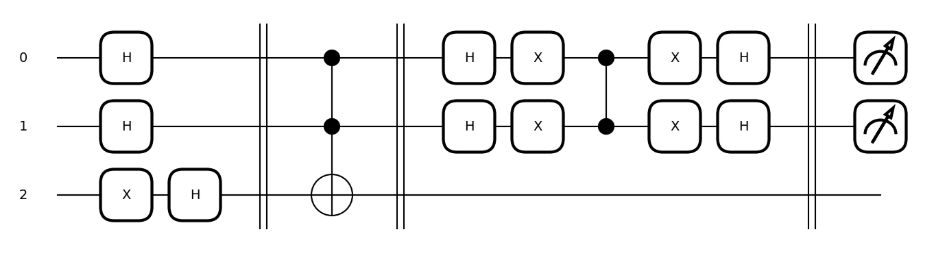
\includegraphics[width=1\textwidth]{image4.png}
    \caption{Exemplo de uma iteração do algoritmo com dois bits em que o $R = 1$}
    \label{fig:minha_imagem}
\end{figure}

\section{Conclusão: A Intersecção com a Criptografia}
A existência e a eventual implementação prática em larga escala dos algoritmos de Grover e de Shor possuem implicações profundas e imediatas no campo da segurança da informação, redefinindo o futuro da criptografia.

A criptografia assimétrica moderna (de chave pública), que sustenta a segurança da internet através de protocolos como RSA e Criptografia de Curva Elíptica (ECC), baseia-se exatamente na dificuldade matemática de fatorar grandes números primos e de resolver logaritmos discretos. A viabilidade prática do \textbf{Algoritmo de Shor} significa que essas defesas clássicas podem ser completamente quebradas por um computador quântico suficientemente robusto e tolerante a falhas, tornando dados criptografados vulneráveis à interceptação e decodificação retroativa.

Por outro lado, a criptografia simétrica (como o padrão AES) não é quebrada tão facilmente, mas é enfraquecida pelo \textbf{Algoritmo de Grover}. A aceleração quadrática de Grover na busca exaustiva (força bruta) significa que o espaço de chaves efetivo de um algoritmo é reduzido à sua raiz quadrada. Na prática, isso exige que o tamanho das chaves simétricas seja dobrado para manter o mesmo nível de segurança pré-quântico (por exemplo, a transição recomendada do AES-128 para o AES-256).

\end{document}